\chapter{Majorization and Momentum}\label{chap:momentum}

\Cref{chap:lyapunov} ended with a negative verdict on descent.  The potential
$\log x$ decreases on average along a Collatz orbit, but it does not decrease
along every stride, and no increasing function of $x$, however it is
reparametrized or majorized, can repair this.  Half of all odd integers ascend
in a single stride, and ascending strides can be chained to any length.  An
optimizer who met an iteration with these properties would not conclude that
it fails to converge.  She would conclude that it is not a descent method, and
she would reach for the other great family of first order methods, the
momentum\index{momentum} methods, whose iterates are allowed to overshoot and whose
convergence is certified by a potential that is not monotone in the objective.

This chapter takes that step.  We review the two classical momentum methods,
Polyak\index{Polyak, B. T.}'s heavy ball\index{heavy ball} method~\cite{polyak1964} and Nesterov\index{Nesterov, Yu.}\index{Nesterov acceleration}'s accelerated
gradient method~\cite{nesterov1983}, with their rates on strongly convex
quadratics and the optimal coefficient $(\sqrt\kappa-1)/(\sqrt\kappa+1)$, and
we recall the continuous time view of Su\index{Su, W.}, Boyd\index{Boyd, S.} and Cand\`es\index{Candes, E. J.@Cand\`es, E. J.}~\cite{su2016} and
Shi\index{Shi, B.}, Du\index{Du, S. S.}, Jordan\index{Jordan, M. I.} and Su~\cite{shi2022}, in which momentum is a damped
oscillator and the certificate\index{certificate} of convergence is an energy that includes a
kinetic term.  We then read the Collatz orbit in the same terms: the odd step
is a momentum injection that overshoots, and the run of halvings that follows
is the correction.  Matching the two pictures produces a small set of
constants, and the main business of the chapter is to say precisely which of
them mean something and which do not.

Three conclusions emerge.  The first is a set of stride constants
(\cref{def:nesterov}) whose ratio $\kappa\approx1.776$, the largest ascent of a
stride over its mean descent, is a ratio of step sizes and not a condition
number\index{condition number} (\cref{rem:nesterovlimits}).  The second is a cautionary
tale: mixing\index{mixing} constants defined at different levels of the iteration produces
spurious agreements (\cref{rem:ch5:mixing}).  The third is a single
number, $\beta=\lt-1=\log(3/2)/\log 2$, that turns up as an ascent to descent
ratio, as a definitional rewriting\index{rewriting system} of a pair of drift\index{drift} constants, as the
excess over one of the Ces\`aro threshold of \cref{chap:divergence}, and as a
ratio of Kullback\index{Kullback and Leibler divergence} and Leibler divergences.  These are one fact seen four
ways, and the number becomes the momentum coefficient of \cref{chap:smm}.
Parrondo\index{Parrondo paradox}'s paradox supplies an analogy along the way.

\section{Momentum methods}\label{sec:ch5:momentum}

Let $f:\R^d\to\R$ be $\mu$ strongly convex with $L$ Lipschitz gradient, and
write $\kappa=L/\mu\ge1$ for its condition number\index{condition number}.  The model case, and the
only one we need for rates, is the quadratic
\begin{equation}\label{eq:ch5:quad}
  f(x)=\tfrac12(x-x^\ast)^{\top}A(x-x^\ast),\qquad
  \mu I\preceq A\preceq LI .
\end{equation}
Gradient descent $x_{t+1}=x_t-\alpha\nabla f(x_t)$ acts on the component of
the error $e_t=x_t-x^\ast$ along an eigenvector with eigenvalue $\lambda$ by
multiplication by $1-\alpha\lambda$.  With $\alpha=1/L$ the worst component,
$\lambda=\mu$, contracts by $1-1/\kappa$ per step; with the best constant step
$\alpha=2/(L+\mu)$ the worst contraction is $(\kappa-1)/(\kappa+1)$.  Either
way the number of iterations needed to reduce the error by a factor
$\varepsilon$ is of order $\kappa\log(1/\varepsilon)$.  Momentum reduces this to
order $\sqrt\kappa\log(1/\varepsilon)$, and the square root is the whole point.

\subsection{Heavy ball}

Polyak~\cite{polyak1964} proposed adding to the gradient step a fraction of the
previous displacement,
\begin{equation}\label{eq:ch5:hb}
  x_{t+1}=x_t-\alpha\nabla f(x_t)+\beta(x_t-x_{t-1}),
\end{equation}
and showed that on the quadratic \eqref{eq:ch5:quad} the choice
\begin{equation}\label{eq:ch5:hbtune}
  \alpha=\frac{4}{(\sqrt L+\sqrt\mu)^2},\qquad
  \beta=\Bigl(\frac{\sqrt\kappa-1}{\sqrt\kappa+1}\Bigr)^2
\end{equation}
makes the spectral radius of the two step recursion equal to
$(\sqrt\kappa-1)/(\sqrt\kappa+1)$~\cite{polyak1987}, which matches the lower
bound of Nesterov\index{Nesterov acceleration} for first order methods on strongly convex quadratics in
high dimension~\cite{nesterov2004}.  The guarantee is a statement about
quadratics, and more generally about a neighbourhood of a nondegenerate
minimum.  It does not extend globally: Lessard\index{Lessard, L.}, Recht\index{Recht, B.} and
Packard\index{Packard, A.}~\cite{lessard2016} exhibit a strongly convex function on which heavy
ball with the tuning \eqref{eq:ch5:hbtune} fails to converge, settling
instead into a limit cycle.  Momentum that is too aggressive for the global geometry
can produce a limit cycle, a phrase the reader of \cref{chap:cycles} will
recognize.

\subsection{Nesterov acceleration}

Nesterov\index{Nesterov acceleration}~\cite{nesterov1983} moved the gradient evaluation to an extrapolated
point,
\begin{equation}\label{eq:ch5:nag}
  y_t=x_t+\beta_t(x_t-x_{t-1}),\qquad x_{t+1}=y_t-\alpha\nabla f(y_t).
\end{equation}
For merely convex $f$ and a momentum\index{momentum} sequence $\beta_t$ that tends to one like
$1-3/t$, with $\alpha=1/L$, the method achieves
$f(x_t)-f^\ast=O(L\|x_0-x^\ast\|^2/t^2)$, against $O(1/t)$ for gradient
descent, and this order cannot be improved by any first order method in the
worst case~\cite{nesterov2004}.  For strongly convex $f$ one uses a constant
coefficient.  The next proposition gives the optimal constant on quadratics
with a complete proof, since it is the formula that \cref{chap:smm} sets out
to avoid.

\begin{proposition}[Optimal constant momentum on quadratics]\label{prop:ch5:nagquad}
Let $f$ be the quadratic \eqref{eq:ch5:quad} with spectrum in $[\mu,L]$, and
run \eqref{eq:ch5:nag} with $\alpha=1/L$ and constant $\beta\in[0,1)$.  On the
eigendirection with eigenvalue $\lambda$, put $a=\lambda/L\in[1/\kappa,1]$.
Then the error obeys a linear two step recursion with characteristic
polynomial
\begin{equation}\label{eq:ch5:charpoly}
  p_a(z)=z^2-(1-a)(1+\beta)z+(1-a)\beta .
\end{equation}
Let $r(\beta)=\max_{a\in[1/\kappa,1]}\rho_a(\beta)$, where $\rho_a$ is the
largest modulus of a root of $p_a$.  Then $r$ is minimized at
\begin{equation}\label{eq:ch5:betaopt}
  \beta^{\mathrm{opt}}(\kappa)=\frac{\sqrt\kappa-1}{\sqrt\kappa+1},
  \qquad\text{with}\qquad r\bigl(\beta^{\mathrm{opt}}\bigr)=1-\frac1{\sqrt\kappa}.
\end{equation}
\end{proposition}

\begin{proof}
On the eigendirection, $y_t=(1+\beta)e_t-\beta e_{t-1}$ and
$e_{t+1}=(1-a)y_t$, which gives \eqref{eq:ch5:charpoly}.  Write $c=1-a$.  The
roots of $p_a$ are real when $\Delta=c(1+\beta)^2-4\beta\ge0$ and complex
conjugate with modulus $\sqrt{c\beta}$ otherwise.

First fix $a=1/\kappa$, so $c=1-1/\kappa$, and regard $\Delta$ as a quadratic in
$\beta$.  Its roots have product one, and a direct substitution shows that
$\beta^{\mathrm{opt}}$ is one of them: $(1+\beta^{\mathrm{opt}})^2=
4\kappa/(\sqrt\kappa+1)^2$, so $c(1+\beta^{\mathrm{opt}})^2=
4(\kappa-1)/(\sqrt\kappa+1)^2=4\beta^{\mathrm{opt}}$.  Hence $\Delta<0$ for
$\beta\in(\beta^{\mathrm{opt}},1)$, where $\rho_{1/\kappa}=\sqrt{c\beta}$ is
increasing in $\beta$; and $\Delta\ge0$ for $\beta\le\beta^{\mathrm{opt}}$, where the
larger root $z_+$ lies below $1$ (because $p_a(1)=a>0$ and the vertex
$c(1+\beta)/2$ is below $1$), and there $\partial p_a/\partial\beta=c(1-z_+)>0$
while $\partial p_a/\partial z=\sqrt{c\Delta}\ge0$, so $z_+$ is nonincreasing in
$\beta$ by implicit differentiation.
Thus $\rho_{1/\kappa}$ is minimized at $\beta^{\mathrm{opt}}$, where $p_{1/\kappa}$ has
the double root
\[
  \sqrt{c\beta^{\mathrm{opt}}}
  =\sqrt{\frac{\kappa-1}{\kappa}\cdot\frac{\sqrt\kappa-1}{\sqrt\kappa+1}}
  =\frac{\sqrt\kappa-1}{\sqrt\kappa}=1-\frac1{\sqrt\kappa}.
\]
Since $r(\beta)\ge\rho_{1/\kappa}(\beta)$, this is a lower bound for $r$.  It is
attained: at $\beta=\beta^{\mathrm{opt}}$ and $a>1/\kappa$ the discriminant is
smaller than at $a=1/\kappa$, hence negative, and the modulus
$\sqrt{(1-a)\beta^{\mathrm{opt}}}$ is smaller than $1-1/\sqrt\kappa$.
\end{proof}

We checked the proposition numerically by minimizing the worst case spectral
radius over a grid of $\beta$ for $\kappa=4$, $14.58$ and $100$ (script
\texttt{ch5\_nag\_check.py}); the minimizers agree with \eqref{eq:ch5:betaopt}
to the grid resolution and the minimal radii are $0.500$, $0.738$ and $0.900$,
as $1-1/\sqrt\kappa$ predicts.  Note the shape of the optimum.  The slowest
direction is tuned to critical damping, a double root, and every faster
direction is underdamped and oscillates.  Accelerated methods converge by
spiralling, and their objective values need not decrease monotonically; the
characteristic ripples of Nesterov's method and the restart schemes designed
to remove them are discussed by O'Donoghue\index{ODonoghue, B.@O'Donoghue, B.} and Cand\`es~\cite{odonoghue2015}.

\section{The continuous time view}\label{sec:ch5:ode}

The heavy ball\index{heavy ball} update is a discretization of a damped oscillator.  Take the
equation
\begin{equation}\label{eq:ch5:oscillator}
  \ddot X+\gamma\dot X+\nabla f(X)=0
\end{equation}
and replace the derivatives by differences with time step $h$:
$(x_{t+1}-2x_t+x_{t-1})/h^2+\gamma(x_t-x_{t-1})/h+\nabla f(x_t)=0$.
Solving for $x_{t+1}$ gives exactly \eqref{eq:ch5:hb} with
\[
  \alpha=h^2,\qquad \beta=1-\gamma h .
\]
The momentum\index{momentum} coefficient is one minus the damping per step.  Critical damping
of the slowest mode of a quadratic, $\gamma=2\sqrt\mu$, with $h=1/\sqrt L$,
gives $\beta=1-2/\sqrt\kappa$, which agrees with
$\beta^{\mathrm{opt}}=1-2/(\sqrt\kappa+1)$ to leading order in $1/\sqrt\kappa$.  So
the optimal coefficient of \cref{prop:ch5:nagquad} is, asymptotically, the
statement that the continuous system should be critically damped in its
slowest direction.

The certificate\index{certificate} of convergence for \eqref{eq:ch5:oscillator} is the energy
\begin{equation}\label{eq:ch5:energy}
\begin{aligned}
  \mathcal E(t)&=f(X(t))-f^\ast+\tfrac12\|\dot X(t)\|^2,\\
  \dot{\mathcal E}&=\dot X^{\top}\bigl(\nabla f(X)+\ddot X\bigr)=-\gamma\|\dot X\|^2\le0 .
\end{aligned}
\end{equation}
The energy decreases, but the objective $f(X(t))$ alone need not: potential
energy is converted to kinetic energy and back, and $f$ can rise while the
ball climbs the far wall of the valley.  This is the structural feature that
\cref{chap:lyapunov} lacked.  There every candidate was an increasing function of the
current position $x$, and \cref{thm:nolyapunov} showed that no such function
can decrease along every stride.  For momentum methods the Lyapunov function\index{Lyapunov function}
lives on the phase space of positions and velocities, and the systematic
construction of such functions for accelerated methods is carried out by
Wilson\index{Wilson, A. C.}, Recht and Jordan~\cite{wilson2021}.  The Collatz analogue of a velocity
would be some memory of the recent parity pattern, which is precisely the
arithmetic information that \cref{rem:ch4:monotone} says a successful
certificate must use.

For Nesterov\index{Nesterov acceleration}'s method Su, Boyd and Cand\`es~\cite{su2016} found the limiting
equation in the convex case, with $\beta_t=(t-1)/(t+2)$, step $s\to0$ and time
$t\sqrt s$:
\begin{equation}\label{eq:ch5:sbc}
  \ddot X+\frac3t\dot X+\nabla f(X)=0,\qquad
  f(X(t))-f^\ast\le\frac{2\|x_0-x^\ast\|^2}{t^2}.
\end{equation}
The damping $3/t$ vanishes as $t\to\infty$, which is why the method keeps
oscillating.  The constant $3$ is not arbitrary: for the family
$\ddot X+(r/t)\dot X+\nabla f(X)=0$ Su, Boyd and Cand\`es identify $r=3$ as a
threshold at which the qualitative behaviour changes.  In the strongly convex case with
constant momentum both heavy ball and Nesterov have the same low resolution
limit, $\ddot X+2\sqrt\mu\,\dot X+\nabla f(X)=0$, and so the limit cannot
explain why Nesterov's method is globally accelerated while heavy ball is not.
Shi, Du, Jordan and Su~\cite{shi2022} resolved this by keeping terms of order
$\sqrt s$.  Their high resolution equations are
\begin{align}
  \text{heavy ball:}\quad&\ddot X+2\sqrt\mu\,\dot X+(1+\sqrt{\mu s})\nabla f(X)=0,
  \label{eq:ch5:hrhb}\\
  \text{Nesterov:}\quad&\ddot X+2\sqrt\mu\,\dot X+\sqrt s\,\nabla^2 f(X)\dot X
  +(1+\sqrt{\mu s})\nabla f(X)=0 .
  \label{eq:ch5:hrnag}
\end{align}
The extra term $\sqrt s\,\nabla^2f(X)\dot X$ is a gradient correction: it
damps the motion more strongly where the curvature is large, and it is the
continuous trace of evaluating the gradient at the extrapolated point rather
than at the current one.  In the language we shall use for the Collatz map,
the extrapolation overshoots and the gradient correction at the overshot point
pulls back.

\section{The Collatz orbit as overshoot and correction}\label{sec:ch5:overshoot}

Under the standard map\index{standard map} $T_0$ an odd $x$ goes to $3x+1$, which is even, so every
odd step is followed by at least one halving (\cref{prop:nocons}).  On the
logarithmic scale the orbit therefore alternates between a single upward jump
of $\log(3+1/x)\approx\log 3$ and a run of $k=\vt(3x+1)\ge1$ downward jumps of
$\log 2$ each.  Grouping the two gives the Syracuse stride, whose increment
$\log(3+1/x)-k\log 2$ was analysed exactly in \cref{thm:stride}.  The picture
has the shape of the one in the previous section, with the roles labelled:
\begin{itemize}
\item the odd step is a \emph{momentum injection}: it moves the potential in
  the wrong direction by a fixed amount, independently of how far the orbit is
  from its target;
\item the halvings are the \emph{correction}: each lowers the potential by the
  same amount, and their number is decided by the arithmetic of $3x+1$, not by
  the size of the overshoot.
\end{itemize}
The second point is where the analogy is weakest and also where it is most
suggestive.  In a momentum\index{momentum} method the correction is computed from the gradient
at the overshot point, so it responds to the overshoot.  In the Collatz map the
number of halvings is $\vt(3x+1)$, which depends only on the residue of $x$ modulo a power of $2$, and in the
model, where successive halving exponents are independent draws from the
Geometric$(\tfrac12)$ law of \cref{prop:geom}, it is independent of the
past.  The correction is blind, and the conjecture asserts that blind
corrections nevertheless dominate along every orbit.

\begin{example}[The orbit of $27$ as injections and corrections]\label{ex:ch5:27}
The orbit of $27$ under $T_0$ reaches $1$ after $111$ steps, of which $41$ are
odd steps and $70$ are halvings, and it climbs as high as $9232$ on the way.
Grouped into strides it consists of $41$ Syracuse strides with halving
exponents
\[
\begin{gathered}
  1,2,1,1,1,1,2,2,1,2,1,1,2,1,1,1,2,3,1,1,2,\\
  1,2,1,1,1,1,1,3,1,1,1,4,2,2,4,3,1,1,5,4 .
\end{gathered}
\]
Of the $41$ strides, $24$ have $k=1$ and so ascend by \cref{thm:stride}: more
than half of the corrections are too small to undo their injection, and the
longest run of consecutive ascending strides has length $5$.  The orbit
descends anyway because the remaining $17$ strides carry large exponents.  The
average number of halvings per odd step is $\bar k=70/41=1.7073$, and the
orbit satisfies $70\log2=48.520>41\log3+\log 27=48.339$, the inequality that
\cref{prop:cesaro} forces on every orbit that reaches $1$.  The margin is
small: about $0.18$ on the logarithmic scale out of $48.5$.  (Script
\texttt{ch5\_numbers.py}.)
\end{example}

\section{Stride constants}\label{sec:ch5:stride}

An accelerated method converges at a rate governed by the ratio of the
largest to the smallest curvature.  The stride descent theorem has the same
two sided shape, an ascent in case (iii) and a descent in case (ii), so it is
natural to form the corresponding ratio.  The quantities must be defined at
the same level of the iteration, and the stride is the natural level, since it
is the smallest unit that contains both an injection and its correction.

\begin{definition}[Stride constants]\label{def:nesterov}
For the Syracuse map\index{Syracuse map} $S$ on odd integers $x\ge3$ put
\begin{align*}
  L&:=\sup_{x\ \mathrm{odd},\ x\ge3}\bigl(\log S(x)-\log x\bigr)=\log\tfrac53=0.5108,\\
  \mu&:=-\E\bigl[\log S(x)-\log x\bigr]=\bigl|\log\tfrac34\bigr|=0.2877,
\end{align*}
where the expectation is under the Geometric$(\tfrac12)$ law of
$k=\vt(3x+1)$ with the correction $\log(1+1/(3x))$ neglected.  The
\emph{stride ratio} is $\kappa:=L/\mu=1.776$.
\end{definition}

The supremum is attained at $x=3$, where $S(3)=5$, by \cref{thm:stride}(iii);
the mean was computed in \cref{sec:ch4:stride}.
To four decimal places, $\kappa=1.7757$, and the \emph{Nesterov\index{Nesterov acceleration} style rate} $1-\kappa^{-1/2}$ that one may form from it by analogy with \cref{prop:ch5:nagquad} is $0.2496$.
If one insisted on the formula of
\cref{prop:ch5:nagquad}, the optimal coefficient at this $\kappa$ would be
$(\sqrt\kappa-1)/(\sqrt\kappa+1)=0.143$.

\begin{remark}[What this is and is not]\label{rem:nesterovlimits}
$L$ is the largest ascent that a single stride can produce and $\mu$ is the
mean descent per stride.  Both are increments of the potential $\log x$ at
the same level of the iteration, which is what makes their ratio
dimensionless and meaningful as a comparison of step sizes.  Neither is a
curvature bound.  $L$ is not the Lipschitz constant of a gradient and $\mu$ is
not a strong convexity modulus, because there is no gradient and no convex
objective: the Collatz map does not minimize anything by evaluating
derivatives.  Consequently $\kappa$ is a ratio of increments rather than a
condition number\index{condition number}, and the rate $1-\kappa^{-1/2}$ is an analogy with no
theorem behind it.  No result in this book uses it.  We report it because it
is the natural dimensional comparison and because it fixes an order of
magnitude: the largest net ascent of a stride is less than twice the mean net descent per stride.

The number is also sensitive to conventions that have no optimization
meaning.  The supremum $L$ is attained only at $x=3$; removing that single point moves it to $\log(11/7)$, attained at $x=7$, and the ratio to $1.571$ (rate $0.202$).
Using instead the
asymptotic ascent $\log(3/2)$ of a stride with $k=1$ and large $x$ gives
$\log(3/2)/\log(4/3)=1.409$ and a rate $0.158$.  A genuine condition number
does not move when a single point is removed from the domain.
\end{remark}

\begin{remark}[A pitfall: mixing levels]\label{rem:ch5:mixing}
One might take for $L$ the ascent of the bare odd step $x\mapsto3x+1$,
whose largest value over odd $x\ge3$ is $\log(10/3)=1.204$, while keeping the
per stride mean descent $\mu=|\log(3/4)|$.  The ratio is then
$\log(10/3)/|\log(3/4)|=4.185$ and the Nesterov style rate is
$1-4.185^{-1/2}=0.511$.  This number is close to $0.52$, the modulus of the
second eigenvalue of the chain on residues modulo $27$ of
\cref{rem:ch9:oddreps} when its states are restricted to the nine odd
representatives of the units in $[1,27)$.  An
agreement between a rate derived from the potential and a rate derived from
the residue dynamics would be remarkable if it were real.

It is not real.  The mixed ratio compares an ascent defined at the level of a
single step of $T_0$ with a descent defined at the level of a stride, and it
corresponds to no consistent picture of the iteration; with the levels
matched as in \cref{def:nesterov} the rate is $0.250$ and there is nothing to
match.  The value $0.52$ is an artefact of a different kind.  Since $27$ is
odd, every residue class modulo $27$ contains integers of both parities, so
the nine states are not a set of odd residues; the chain leaves them with
positive probability, and conditioning on a set that is not invariant produces
spurious eigenvalues.  The model chain on all eighteen units, with independent
Geometric$(\tfrac12)$ halving exponents, is exactly stationary\index{mixing} after three
strides, by an identity of Tao\index{Tao, T.}~\cite[eq.~(1.21)]{tao2022}, and so every
eigenvalue other than $1$ is zero (\cref{lem:ch9:mixing}).  The same lesson applies to the matched rate itself:
its value $0.2496$ lies within $0.0005$ of $1-e^{-\mu}=1/4$, the
fractional decrease per stride of the geometric mean of $x$ in the model, and
this closeness is equally accidental, since $\kappa^{-1/2}$ and $e^{-\mu}$ are
unrelated functions of the constants.  With a handful of constants of order one and a tolerance of
a few percent, coincidences are to be expected, and none of them should be
reported as a finding.
\end{remark}

\section{Per step and per macro step constants}\label{sec:ch5:perstep}

A second pair of constants is natural if one looks at the accelerated map
$T(x)=x/2$ or $(3x+1)/2$ of \cref{def:maps} rather than at strides.  Every step
of $T$ changes $\log x$ by $-\log 2$ if $x$ is even and by
$\log(3/2+1/(2x))\in(\log(3/2),\log2]$ if $x$ is odd, with $\log 2$ attained
only at $x=1$; over odd $x\ge3$ the largest ascent is $\log(5/3)$, at $x=3$, which is the stride constant $L$, since $T(3)=S(3)=5$.
Put
\begin{equation}\label{eq:ch5:star}
  L_\ast:=\log 2=0.6931,\quad
  \mu_\ast:=\bigl|\log\tfrac34\bigr|=0.2877,\quad
  \kappa_\ast:=\frac{L_\ast}{\mu_\ast}=2.409 .
\end{equation}
Here $L_\ast$ is the size of one halving, and also the largest one step ascent of $T$, but only because $x=1$ is admitted; over the odd $x\ge3$ used in the other rows of \cref{tab:ch5:levels} the ratio would be $\kappa$ itself.
Read as an ascent, $L_\ast$ is a per step extremal
quantity, while $\mu_\ast$ is the mean descent per Syracuse macro step under
the Geometric$(\tfrac12)$ law, a per macro step expectation.
The ratio $\kappa_\ast$ therefore pairs quantities defined at different levels, as in \cref{rem:ch5:mixing}, but its excess over $\kappa$ comes entirely from the point $x=1$.
\Cref{tab:ch5:levels} collects the three ratios side by side.

\begin{table}[t]
\centering
\caption{Ratios of an ascent constant to a descent constant at different
levels of the iteration. Only the first row compares quantities defined at
the same level. The rate column is $1-\kappa^{-1/2}$ in each case and has no
theorem behind it. The ascent $\log(10/3)$ is the largest over odd $x\ge3$; at
$x=1$ the step $1\mapsto4$ ascends by $\log4$.
The ascent $\log2$ is attained only at $x=1$; over odd $x\ge3$ a step of $T$ ascends by at most $\log(5/3)$, as in the first row.}
\label{tab:ch5:levels}
\small\setlength{\tabcolsep}{4pt}
\begin{tabular}{lllcc}
\toprule
Ascent & Level & Descent & $\kappa$ & $1-\kappa^{-1/2}$\\
\midrule
$\log(5/3)$ & stride & $|\log(3/4)|$ per stride & $1.776$ & $0.250$\\
$\log 2$ & step of $T$ & $|\log(3/4)|$ per stride & $2.409$ & $0.356$\\
$\log(10/3)$ & step of $T_0$ & $|\log(3/4)|$ per stride & $4.185$ & $0.511$\\
\bottomrule
\end{tabular}
\end{table}

The pair $(L_\ast,\mu_\ast)$ has one virtue, which is also a trap.  Since
$\log(3/4)=\log3-2\log2$,
\begin{equation}\label{eq:ch5:definitional}
  1-\frac{\mu_\ast}{L_\ast}
  =1-\frac{2\log2-\log3}{\log2}
  =\frac{\log3-\log2}{\log2}
  =\frac{\log(3/2)}{\log 2}
  =:\beta .
\end{equation}
The left side has the form $1-1/\kappa_\ast$, and an optimizer will recognize
in it a familiar way of writing a momentum\index{momentum} coefficient in terms of a condition
number.  One might read \eqref{eq:ch5:definitional} as a discovery,
namely that the Collatz map selects its own momentum coefficient.  It is
nothing of the kind.  It is a definitional identity, a rearrangement of
$\log(3/4)=\log 3-2\log 2$, and it would hold for any pair of constants so
defined; \cref{rem:ch6:definitional} returns to it from the optimizer's side.
Equivalently $1/(1-\beta)=\kappa_\ast$, and when this quantity reappears in
\cref{chap:noise} as the slow mode noise amplification of every step momentum
at coefficient $\beta$, it is the same algebra again.

\begin{remark}[Another definitional coincidence]\label{rem:ch5:clt}
By \cref{prop:ch5:nagquad}, a fixed coefficient $\beta$ is optimal for exactly
one condition number\index{condition number}, $\kappa=\bigl((1+\beta)/(1-\beta)\bigr)^2$.  For
$\beta=\log(3/2)/\log2$ we have $(1+\beta)/(1-\beta)=\log3/\log(4/3)$, so this
condition number is
\[
  \Bigl(\frac{\log 3}{\log(4/3)}\Bigr)^2=14.58 .
\]
The same number appears in \cref{chap:stochastic} as the constant
$C=\sigma^2/(\ds)^2$ that sets the scale of the central limit theorem\index{central limit theorem} for
stopping times.  Again the coincidence is algebraic.  Under the Bernoulli model\index{Bernoulli model} a
step of $T$ is a fair choice between $\log(3/2)$ and $-\log 2$, so its standard
deviation is half the gap, $\sigma=\tfrac12\log 3$, and its mean is
$\ds=\tfrac12\log(3/4)$; the ratio $\sigma/|\ds|$ is
$\log3/\log(4/3)=(1+\beta)/(1-\beta)$ by the same rearrangement as
\eqref{eq:ch5:definitional}.  Two quantities built from $\log 2$ and $\log 3$
in the same way are equal; nothing more follows.
\end{remark}

\section{One number in four places}\label{sec:ch5:beta}

Set aside the condition number\index{condition number} language, which does not survive scrutiny, and
look at the number itself:
\begin{equation}\label{eq:ch5:beta}
  \beta=\frac{\log(3/2)}{\log 2}=\lt-1=0.584963\ldots
\end{equation}
It is the fractional part of $\lt$, whose continued fraction\index{continued fraction} expansion governs
the cycle problem of \cref{chap:cycles}.  It appears in four guises in this
book, and they are a single fact.

\paragraph{As an ascent to descent ratio.}  An odd step of the accelerated map $T$
raises the potential by $\log(3/2)+O(1/x)$, and a halving lowers it by
$\log 2$.  Measured in units of one halving, the overshoot of an injection is
$\beta$, asymptotically.  In the standard map\index{standard map} $T_0$ the odd step has not yet
absorbed its first halving, and its overshoot in the same units is
$\lt=1+\beta$.

\paragraph{As a Ces\`aro threshold.}  Along an orbit of odd iterates
$y_0,y_1,\dots$ with halving exponents $k_j$, the average $\bar k_N$ is the
number of halvings per odd step.  Every orbit that
reaches $1$ from $x_0>1$ has $\bar k_N>\lt$ at the stride $N$ at which it reaches $1$ (\cref{prop:cesaro}), and an unbounded orbit has
$\limsup\bar k_N\le\lt$ (\cref{cor:ch9:freq}).  So the threshold for halvings per odd step is
exactly the overshoot of one injection measured in halvings,
\[
  \bar k>1+\beta ,
\]
which is the statement that corrections outweigh injections on average,
counted in the same units.  Under the Geometric$(\tfrac12)$ law $\E k=2$, and
the margin is $2-(1+\beta)=1-\beta=\mu_\ast/L_\ast=0.415$, a margin that
describes the model, in which $k$ is evaluated at a uniformly random odd
residue; along an unbounded orbit the identity leaves no margin at all.  The
orbit of $27$ in \cref{ex:ch5:27} has $\bar k=1.707$, above $1.585$, as every
orbit that reaches $1$ must be, and well below the model mean.  \Cref{chap:divergence} reduces the divergence half of
the conjecture to a lower bound on $\liminf\bar k_N$ of exactly this form
(\cref{conj:cesaro}).

\paragraph{As a rewriting of drift constants.}  This is
\eqref{eq:ch5:definitional}, and we have said what it is worth: the per macro
step drift\index{drift} $\log(3/4)$ equals $(\beta-1)\log2$, so the drift is negative
because $\beta<1$, and $\beta<1$ is the statement $3<4$.

\paragraph{As a ratio of divergences.}  Let $U_j$ be the uniform law on a set
of $j$ points, with $U_1\subset U_2\subset U_3$ nested in the sense of
supports.  Then $\KL(U_j\,\|\,U_{j+1})=\log\bigl((j+1)/j\bigr)$, since each of
the $j$ atoms of $U_j$ contributes $\tfrac1j\log\bigl((j+1)/j\bigr)$, and
therefore
\begin{equation}\label{eq:ch5:kl}
  \frac{\KL(U_2\,\|\,U_3)}{\KL(U_1\,\|\,U_2)}=\frac{\log(3/2)}{\log 2}=\beta .
\end{equation}
\Cref{lem:ch6:kl} states this formally and discusses its Sanov reading; here
we note only how it connects to the other three guises.
An odd step of $T$ multiplies by $3/2$ and a halving divides by $2$, so the potential moves by $\log(3/2)$ and by $\log2$.
These are exactly the divergences in \eqref{eq:ch5:kl}, the information lost in compressing three equally likely states to two and two to one, and their ratio is the ratio of the two moves.
The integers $2$ and $3$ do all the work in
every guise, which is why the four agree.

\section{Parrondo's paradox}\label{sec:ch5:parrondo}

The Collatz iteration alternates two moves with opposite effects on the
potential, and which move is made is decided by the state, through its
parity.  A well known family of games has the same architecture and a
surprising conclusion.
Parrondo\index{Parrondo paradox}'s games, devised by Parrondo\index{Parrondo, J. M. R.} and published by Harmer\index{Harmer, G. P.} and Abbott\index{Abbott, D.}~\cite{harmer1999statsci,harmer1999}, show that two games, each losing when
played alone, can combine to make a winning one.

The capital dependent version runs as follows.  A player's capital changes by
$\pm1$ at each play.  In game A a coin with winning probability $\tfrac12-\epsilon$
is tossed.  In game B the coin depends on the capital: if the capital is a
multiple of $3$ the winning probability is $\tfrac1{10}-\epsilon$, and otherwise it
is $\tfrac34-\epsilon$.  Game A is plainly losing for $\epsilon>0$.  Game B is a
Markov chain on the capital modulo $3$, and its long run gain per play is
$\sum_s\pi_s(2p_s-1)$, where $\pi$ is the stationary law of the residue and
$p_s$ the winning probability in state $s$.  We computed these quantities
exactly (script \texttt{ch5\_parrondo.py}); \cref{tab:ch5:parrondo} gives
the results.

\begin{table}[t]
\centering
\caption{Long run gain per play in the capital dependent Parrondo games.
Random mixture: A or B chosen by a fair coin at each play. Periodic patterns
are repeated indefinitely. Exact stationary computations; a simulation of
$2\times10^6$ plays of AABB at $\epsilon=0.005$ gave $0.0138$.}
\label{tab:ch5:parrondo}
\begin{tabular}{lcc}
\toprule
Game & $\epsilon=0$ & $\epsilon=0.005$\\
\midrule
A alone & $0$ & $-0.0100$\\
B alone & $0$ & $-0.0087$\\
random mixture of A and B & $18/709=0.0254$ & $0.0157$\\
periodic AABB & $0.0245$ & $0.0147$\\
periodic ABB & $0.0679$ & $0.0574$\\
\bottomrule
\end{tabular}
\end{table}

The mechanism is visible in game B at $\epsilon=0$.  If the residue of the
capital modulo $3$ were uniformly distributed, the gain per play would be
$\tfrac13(2\cdot\tfrac1{10}-1)+\tfrac23(2\cdot\tfrac34-1)=\tfrac1{15}>0$.
But the residue is not uniform: the bad state $0$ has stationary probability
$\pi_0=5/13$ rather than $1/3$, and the gain is exactly
$\tfrac5{13}(-\tfrac45)+\tfrac8{13}\cdot\tfrac12=0$.  The state dependent rule
steers the chain towards the state in which it loses.  Interleaving game A
randomizes the capital, pushes the residue law back towards uniform
($\pi_0=245/709$ for the fair mixture), and lets the favourable states of B pay
off.

For the Collatz map the analogy reads as follows.  The ascent move (the odd
step) and the descent move (a halving) are the two games; the first loses for
a player whose aim is to reach $1$, the second wins, and the switching between
them is dictated by the state through its residues modulo powers of $2$.  The
heuristic that the orbit descends computes the long run drift\index{drift} under the
assumption that these residues are uniformly distributed, which is what the
Geometric$(\tfrac12)$ law expresses.  Parrondo's games show, with exact
arithmetic, how far that kind of computation can be from the truth when the
switching rule is coupled to the state: the uniform residue heuristic says
$+1/15$ for game B and the truth is $0$.  An orbit that diverged would be an
orbit whose state dependent switching steered it, in the manner of game B,
into the residues where halvings are scarce, so that $\bar k$ stayed at or
below $1+\beta$.  The statement that this cannot happen is a statement about
the distribution of residues along deterministic orbits, which is the subject
of the Ces\`aro liminf conjecture\index{Cesaro conjecture@Ces\`aro conjecture}, \cref{conj:cesaro};
the residue chains of \cref{chap:divergence} answer the
corresponding question for the model, in which the halving exponents are drawn
independently, and not for a single orbit.

The analogy has limits.  In Parrondo's games both components lose and the
combination wins; in the Collatz map one move ascends and one descends, and
there is no paradox in their combination descending.  What carries over is the
lesson: the long run drift of a state switched system\index{switched system} is a property of the
stationary law of the switching state, not of the components.  The optimizer
of \cref{chap:smm}, which alternates a noise amplifying momentum\index{momentum} step with a
plain gradient step, is governed by the same lesson in a benign form.

\section{Towards Switching MM}\label{sec:ch5:towards}

\Cref{prop:ch5:nagquad} makes the dependence of momentum\index{momentum} on curvature
explicit: the optimal constant coefficient $(\sqrt\kappa-1)/(\sqrt\kappa+1)$ is
an increasing function of the condition number\index{condition number}, near zero for well conditioned
problems and near one for badly conditioned ones.  Any fixed coefficient is
therefore optimal for exactly one $\kappa$.  \Cref{fig:ch5:nesterov} plots the
optimal coefficient against $\kappa$ together with the two fixed values that
will matter in \cref{chap:smm,chap:noise}: the Collatz value
$\beta=0.585$ and the machine learning default $0.9$.  Solving
$(\sqrt\kappa-1)/(\sqrt\kappa+1)=\beta$ gives $\kappa=((1+\beta)/(1-\beta))^2$, so
the crossings are at $\kappa=14.58$ for $\beta=0.585$ and at exactly
$\kappa=361$ for $\beta=0.9$ (script \texttt{ch4\_ch5\_numbers.py}).  The three
ratios of \cref{tab:ch5:levels} are marked for reference only; all three lie in the
region where the optimal coefficient is small, but since none of them is a
condition number (\cref{rem:nesterovlimits}), this says only that the largest
ascent is a small multiple of the mean descent.

\begin{figure}[t]
\centering
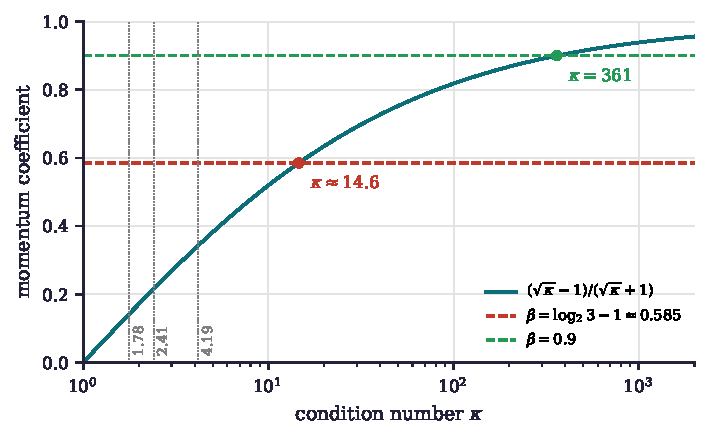
\includegraphics[width=\textwidth]{figures/ch5_nesterov_beta.pdf}
\caption{The optimal constant Nesterov coefficient
$(\sqrt\kappa-1)/(\sqrt\kappa+1)$ on $\kappa$ conditioned quadratics, with the
fixed values $\beta=\lt-1\approx0.585$ and $\beta=0.9$. The crossings, at
$\kappa=((1+\beta)/(1-\beta))^2$, are $\kappa\approx14.6$ and $\kappa=361$. Dotted
vertical lines mark the ratios $1.78$, $2.41$ and $4.19$ of
\cref{tab:ch5:levels}.}
\label{fig:ch5:nesterov}
\end{figure}

The figure states the practitioner's dilemma that opens \cref{chap:smm}: the
optimal coefficient needs $\kappa$, which is usually unknown.  The alternative
pursued there is to fix the coefficient in advance at the number
\eqref{eq:ch5:beta}, the overshoot of an injection measured in corrections.
The figure also shows the price.  The value $0.585$ is the
right amount of momentum only near $\kappa=14.6$ and is too little for harder
problems; \cref{chap:smm} shows that on quadratics the resulting method is not
accelerated at all, and \cref{chap:noise} locates its real advantage
elsewhere, in robustness to noisy gradients.  The second ingredient taken from
the arithmetic is the parity pattern: the Collatz orbit injects only on odd
steps, and Switching MM\index{Switching MM} extrapolates only on odd iterations.  In the language
of this chapter, it is a momentum method whose overshoots are always followed
by a correction, which is the one feature of the Collatz orbit that
\cref{prop:nocons} guarantees.
\Cref{chap:mmcollatz} first presses the majorization idea as far as it will go on the Collatz map itself; \cref{chap:smm,chap:noise} then develop the optimizer, exactly on quadratics and under noise; and \cref{chap:difference}, at the end of Part II, places both objects, the Collatz recursion and the momentum methods, in the common framework of nonlinear difference equations.

\section*{Notes}

The heavy ball\index{heavy ball} method is due to Polyak~\cite{polyak1964}, whose
book~\cite{polyak1987} remains the clearest treatment of momentum\index{momentum} and
Chebyshev\index{Chebyshev step sizes} methods on quadratics.  Nesterov\index{Nesterov acceleration}'s method appeared
in~\cite{nesterov1983}; the lower bounds showing its optimality among first
order methods, and the strongly convex version with constant momentum, are in
his lectures~\cite{nesterov2004}.  The failure of heavy ball to converge
globally on a strongly convex function, and a systematic method for certifying
first order algorithms by small semidefinite programs, are in Lessard, Recht
and Packard~\cite{lessard2016}.  The differential equation
\eqref{eq:ch5:sbc} is from Su, Boyd and Cand\`es~\cite{su2016}, and the high
resolution equations \eqref{eq:ch5:hrhb} and \eqref{eq:ch5:hrnag} from Shi, Du,
Jordan and Su~\cite{shi2022}; Lyapunov functions\index{Lyapunov function} for accelerated methods in
continuous and discrete time are developed systematically by Wilson, Recht and
Jordan~\cite{wilson2021}.  Restarting schemes that suppress the oscillations
of accelerated methods are studied by O'Donoghue and
Cand\`es~\cite{odonoghue2015}.

The stride constants, the per step and per macro step constants and the
identity \eqref{eq:ch5:definitional} are elementary; we present them with the
level of the iteration at which each is defined made explicit, which is the
point of \cref{rem:nesterovlimits,rem:ch5:mixing}.  \Cref{prop:ch5:nagquad} is classical; the proof given here, by
locating the double root, is the standard one.
Parrondo\index{Parrondo paradox}'s games were devised by Parrondo as a pedagogical illustration of the flashing Brownian ratchet; the capital dependent games used here were published by Harmer and Abbott~\cite{harmer1999statsci,harmer1999}, games whose rules depend on the history of play rather than on the capital were introduced by Parrondo, Harmer and Abbott~\cite{parrondo2000}, and~\cite{harmer2002} reviews both; the
observation that game B fails exactly because its residue law is not uniform
is the reason we find the analogy with Collatz parity switching useful.  For the Kullback\index{Kullback and Leibler divergence} and Leibler divergence see any text on
information theory; nothing beyond its definition is used.

\section*{Exercises}

\begin{exercise}
For the heavy ball\index{heavy ball} recursion \eqref{eq:ch5:hb} on a scalar quadratic with
curvature $\lambda$, show that the characteristic polynomial is
$z^2-(1+\beta-\alpha\lambda)z+\beta$.  With the tuning \eqref{eq:ch5:hbtune},
show that both endpoints $\lambda=\mu$ and $\lambda=L$ give double roots of
modulus $(\sqrt\kappa-1)/(\sqrt\kappa+1)$, and that every interior $\lambda$
gives complex roots of modulus $\sqrt\beta$, which is the same number.
\end{exercise}

\begin{exercise}
Verify the energy identity \eqref{eq:ch5:energy}.  For the quadratic
$f(x)=\tfrac12\lambda x^2$ and $\gamma<2\sqrt\lambda$, show that $f(X(t))$ is
not monotone even though $\mathcal E(t)$ is.  Find the analogous discrete
energy for \eqref{eq:ch5:hb} on a scalar quadratic, that is, a positive
definite quadratic form in $(x_t,x_{t-1})$ that decreases along the
iteration whenever the spectral radius is less than one.
\end{exercise}

\begin{exercise}
Compute the stride ratio and the Nesterov\index{Nesterov acceleration} style rate when $L$ is defined as
the supremum of the stride increment over odd $x\ge X$, for $X=3,7,11,\dots$,
and show that the ratio decreases to $\log(3/2)/\log(4/3)=\beta/(1-\beta)$ as
$X\to\infty$.  Explain why this dependence on $X$ is evidence that the stride
ratio is not a condition number\index{condition number}.
\end{exercise}

\begin{exercise}
Let $a,b>0$ with $a<b$ and define $\beta(a,b)=\log(1+a)/\log(1+b)$, the ascent
to descent ratio of a map that multiplies by $1+a$ on one parity class and
divides by $1+b$ on the other.  Show that
$1-\bigl(\log(1+b)-\log(1+a)\bigr)/\log(1+b)=\beta(a,b)$ identically, and
deduce that the identity \eqref{eq:ch5:definitional} holds for every map of
this type.  For which $a$ and $b$ is $\beta(a,b)$ also a ratio
$\KL(U_m\,\|\,U_{m+1})/\KL(U_n\,\|\,U_{n+1})$ of nested uniform divergences?
\end{exercise}

\begin{exercise}
For the capital dependent Parrondo\index{Parrondo paradox} game B with winning probabilities $p_0$ in
state $0$ and $p_1$ in states $1$ and $2$ (capital modulo $3$), show that the
stationary probability of state $0$ is
\[
  \pi_0=\frac{1-p_1+p_1^2}{3-p_0-2p_1+2p_0p_1+p_1^2}.
\]
Hence verify that $\pi_0=5/13$ and the gain is $0$ for $p_0=\tfrac1{10}$,
$p_1=\tfrac34$, and that the fair mixture with game A, which has $p_0=\tfrac3{10}$
and $p_1=\tfrac58$, has $\pi_0=245/709$ and gain $18/709$.
\end{exercise}

\begin{exercise}
For an odd starting value $x_0>1$ whose orbit reaches $1$ after $N$ strides,
show that the number of ascending strides ($k_j=1$) can exceed $N/2$, as it
does for $x_0=27$.  Using \cref{prop:cesaro}, find a lower bound on the
average of $k_j$ over the descending strides in terms of the fraction of
ascending strides, and evaluate it for the orbit of $27$.
\end{exercise}
